% Chapter 2 is usually termed 'Related Work', 'State of the Art' or 'Fundamentals'. Here you will describe
% relevant technologies and standards related to your topic. What did other scientists propose regarding
% your topic? This chapter makes about 20-30 percent of the complete thesis.
%
% This section is intended to give an introduction about relevant terms, technologies
% and standards in the field of X. You do not have to explain common technologies such
% as HTML or XML.
%
% This section describes relevant technologies, starting with X followed by Y, concluding with Z.

\chapter{State of the Art\label{cha:state_of_the_art}}

There are literally two main standards/protocols that are used in this thesis and will be described in
depth in this chapter: the HbbTV standard and the Webdriver protocol. Both are fairly new standards that
have been defined within the last 5 years. Another important protocol for this work is the Chrome Remote
Debugging protocol which is used by the automation driver to drive the Webdriver tests get data out of
the HbbTV app. This thesis tries to connect the standards to allow interoperability between them to
increase the level of integration to a wide variety of tools that has not been possible before.

\section{HbbTV\label{sec:hbbtv}}

% It's always a good idea to explain a technology or a system with a citation of a prominent
% source, such as a widely accepted technical book or a famous person or organization.

Television devices started to become connected to the internet already before HbbTV was invented. With
the so called Set Top Boxes or Smart TV Sticks customers were able to connect the TV to an internet
capable device that provided a content stream. Big companies like Google, Amazon or Apple provided such
devices. The problem with this approach was that if a developer wanted to build an app he had to create
this app for each individual platform. This is a really time consuming and not scaleable process as
the way you build apps for such platforms was extremely different. After game consoles like Sony Playstation
or Microsofts xBox became internet connected devices too there even was another way to transform
the normal TV to a Smart TV. It made it even more difficult for content provider to deploy their services
to all TV platforms.\\
With the open ETSI standard called HbbTV a new way was build to create digital applications for
broadcaster and content provider that runs on every TV supporting that standard. It \textit{''is
a globally initiative technology mainly developed by industry leaders''} \cite{zte}. HbbTV
applications are HTML webpages with additional features that enabled certain interaction between
broadcast and broadband. This means that from a running broadcast stream it allows customers
to open apps that provide additional content to the image on the screen. From that you can start
even more applications that provide different content in non linera fashion. We have to differentiate
here between two different types of apps. There are broadcast-independent applications that are not
connected to any broadcast service and are downloaded and accessed via broadband. The other type are
broadcast-related applications that can be opened when a certain broadcast service is used. They
can start automatically or explicitly upon user request. The advantage of HbbTV here is the independence
to the used device. Content provider can build and deploy apps which can be used by any device if the
standard is supported.\\
If a consumer is equipped with an HbbTV supported Smart TV he will usually see a small image somewhere
on the screen that asks him to press the red button on the remote control. Pressing it triggers an
event within the app that opens the HbbTV application. Once the user switches the channel the same
happens again with a different app. Depending on the broadcaster each broadcast signal contains
a small AIT package that contains main information like application ID, version, autostart state and
application URL of the HbbTV app. Figure \ref{fig:app_delivery} demonstrates the workflow of this
process.

\begin{figure}[htb]
  \centering
  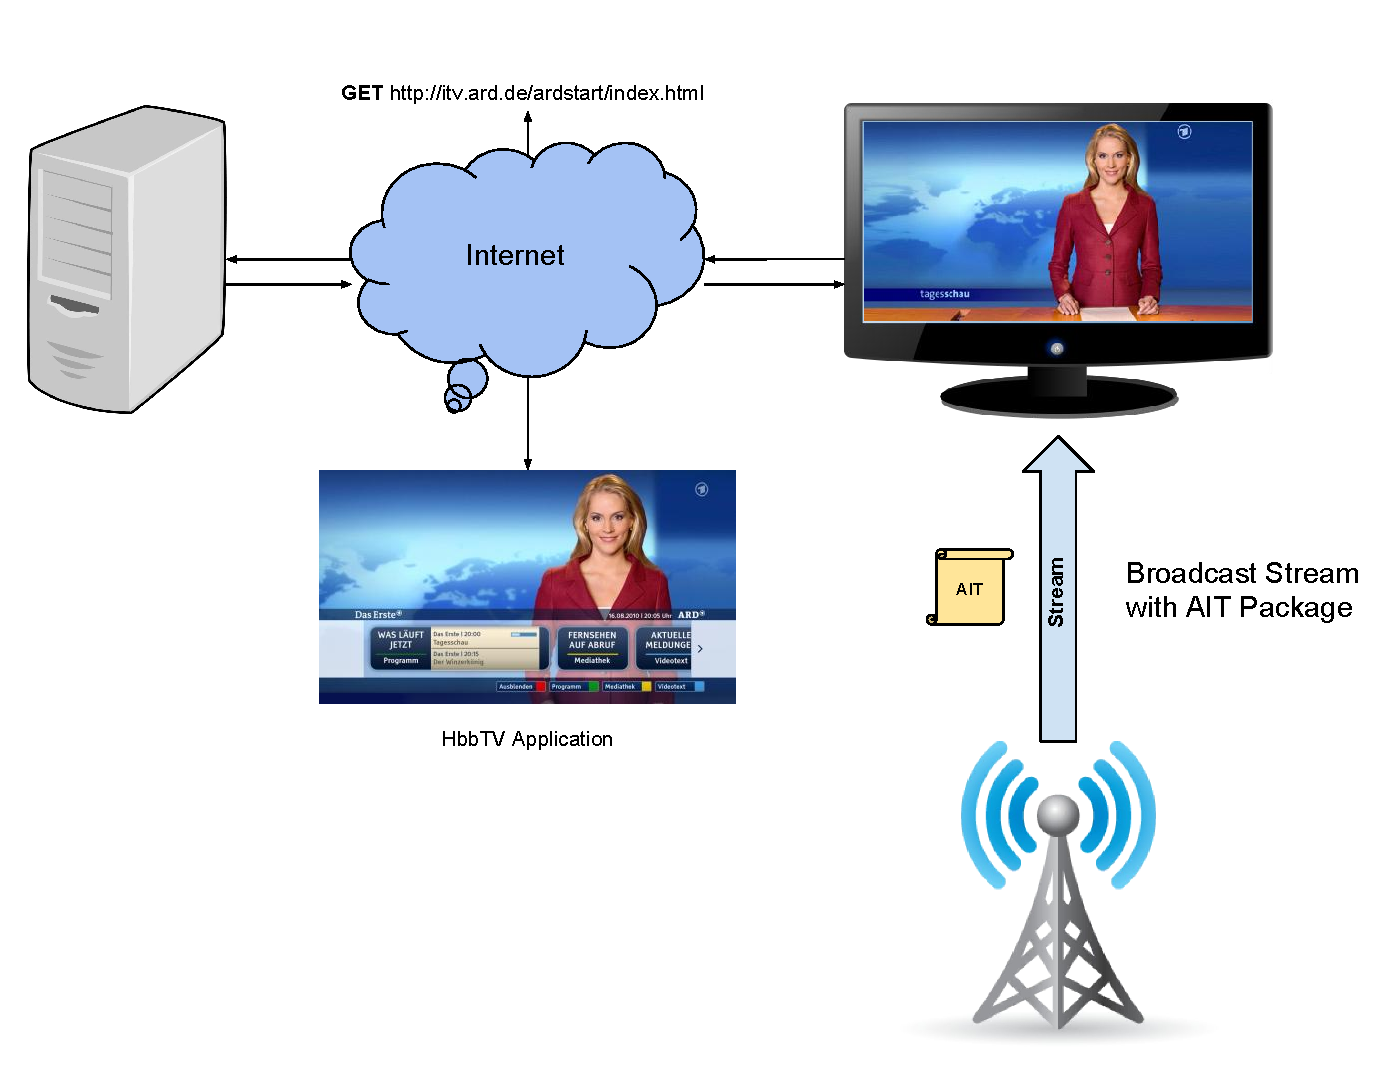
\includegraphics[width=15cm]{app_delivery.pdf}\\
  \caption{App delivery workflow of HbbTV applications}\label{fig:app_delivery}
\end{figure}

Depending on the autostart information within the AIT package the app either starts automatically
as soon as the broadcast stream starts or only when the user pushes the red button. Most HbbTV
applications these days use the autostart feature to display a small indicaticator image to
show that an HbbTV app is available to use. Once the app opens it either takes up only some part
of the screen fulfills the whole display. In general though the broadcast stream is never
getting disrupted as the application only acts as an additional service to the broadcast stream.\\
After the first specification was released in 2010 by the \textit{''HbbTV forum and published by ETSI
in the specification TS 102 796''} \cite{evolution} initiators reached out to CE manufactures to get
it implemented in the next generation of TVs. Since then the number of Smart TVs with HbbTV support
increased drastically with more than 43 million devices sold and over 300 apps deployed in 25
countries\footnote{Source: \url{https://www.hbbtv.org/news-events/hbbtv-ibc-2016-services-and-devices/}}
\footnote{A complete list of all countries can be found in Listing \ref{hbbtvdeployed} in the annex section}.
Alone in Germany there are over 120 HbbTV supported channels\footnote{Source: \url{https://trifinite.org/hbbtv/trifinite_hbbtv_channel_list.html}}
generating roughly 320 million hits monthly\footnote{Source: \url{https://goo.gl/eg8Sfs}}.\\
Almost two years later a new specification was released (HbbTV 1.5) that added support for MPEG DASH
and MPEG CENC. MPEG DASH is an ISO standard for adaptive streaming of IP videos. Depending on the
users bandwith and CPU processing power it ensures continuous playback and helps improving the stream
experience in general by monitoring the CPU utilization and/or buffer status. If e.g. for any reason
the user looses bandwidth the video is able to lower the quality of the video so that it still can
be played without disrupting. Due to support issues not many HbbTV apps use DASH these days.
Most videos are still loaded in a progressiv way. The MPEG CENC on the other side helps with common
encription for ISO base media format files and MPEG-2 transport streams. As content provider using this
feature you only have to encrypt your video once. The user then has to decrypt it by getting the
key from one of many DRM systems.\\
The HbbTV 1.5 standard is supported by the majority of devices these days however many CE manufactures
already are about to support the latest HbbTV spec version 2 with their new devices on the market.
It introduces a lot of new features and supports more web technology standards. While previous HbbTV
apps only work with a version of CE-HTML which is an XHTML-based standard specifically for consumer
electronic devices on UPnP networks, the latest specification supports HTML5, CSS3 and Web Sockets.
Another new feature is the ability for synchronisation of audio, video and data streams that enables
the consumer to watch a certain broadcast stream while listening on the audio via broadband. This
opens a wide variety of use cases like service for simultan translations to videos. It can be
combined with the new introduced Second Screen Integration for Smart Phones and Tablets which
allows to start broadcast streams from your personal handheld on the TV. Due to its duplex
communication ability it allows to also start videos from your HbbTV app on your mobile device.
This works with multiple devices and also provides a lot of opportunities for e.g. gaming applications
where phones can be used as remote controls. In the video area the specifications will support
new streaming formats like HEVC, also known as H.265 and MPEG-H Part 2, DASH for DVB or
push-on-demand where users are able to download certain videos on a local storage to watch them
if desired.\\
It is worth mentioning that version 2 of the spec was never really released by ETSI. It got
surpassed by version 2.0.1 which fixed unclear specifications and removed some errors. It also
shipped some additional specifications that were required to adapt the standard in Italy and United
Kingdom who have decided to move from a similar standard called MHP to HbbTV. These specifications
define additional caching rules for HTTP/1.1, more details on higher display resolution and other
technologies that were defined in MHP.\\
An additional standard to HbbTV was released short after HbbTV version 2 was published by ETSI.
This standard is called Application Discovery over Broadband and is not part of the actual
HbbTV specification. However it adds an important addition to HbbTV when cable service provider block
the AIT of the broadcast stream. These provide have a different idea of interactive TV services
and usually want to promote their own platform. Once the AIT package is blocked the HbbTV application
can't be loaded by the TV anymore since information about application ID and URL are missing.
Application Discovery over Broadband is a workaround to solve this problem.

\begin{figure}[htb]
  \centering
  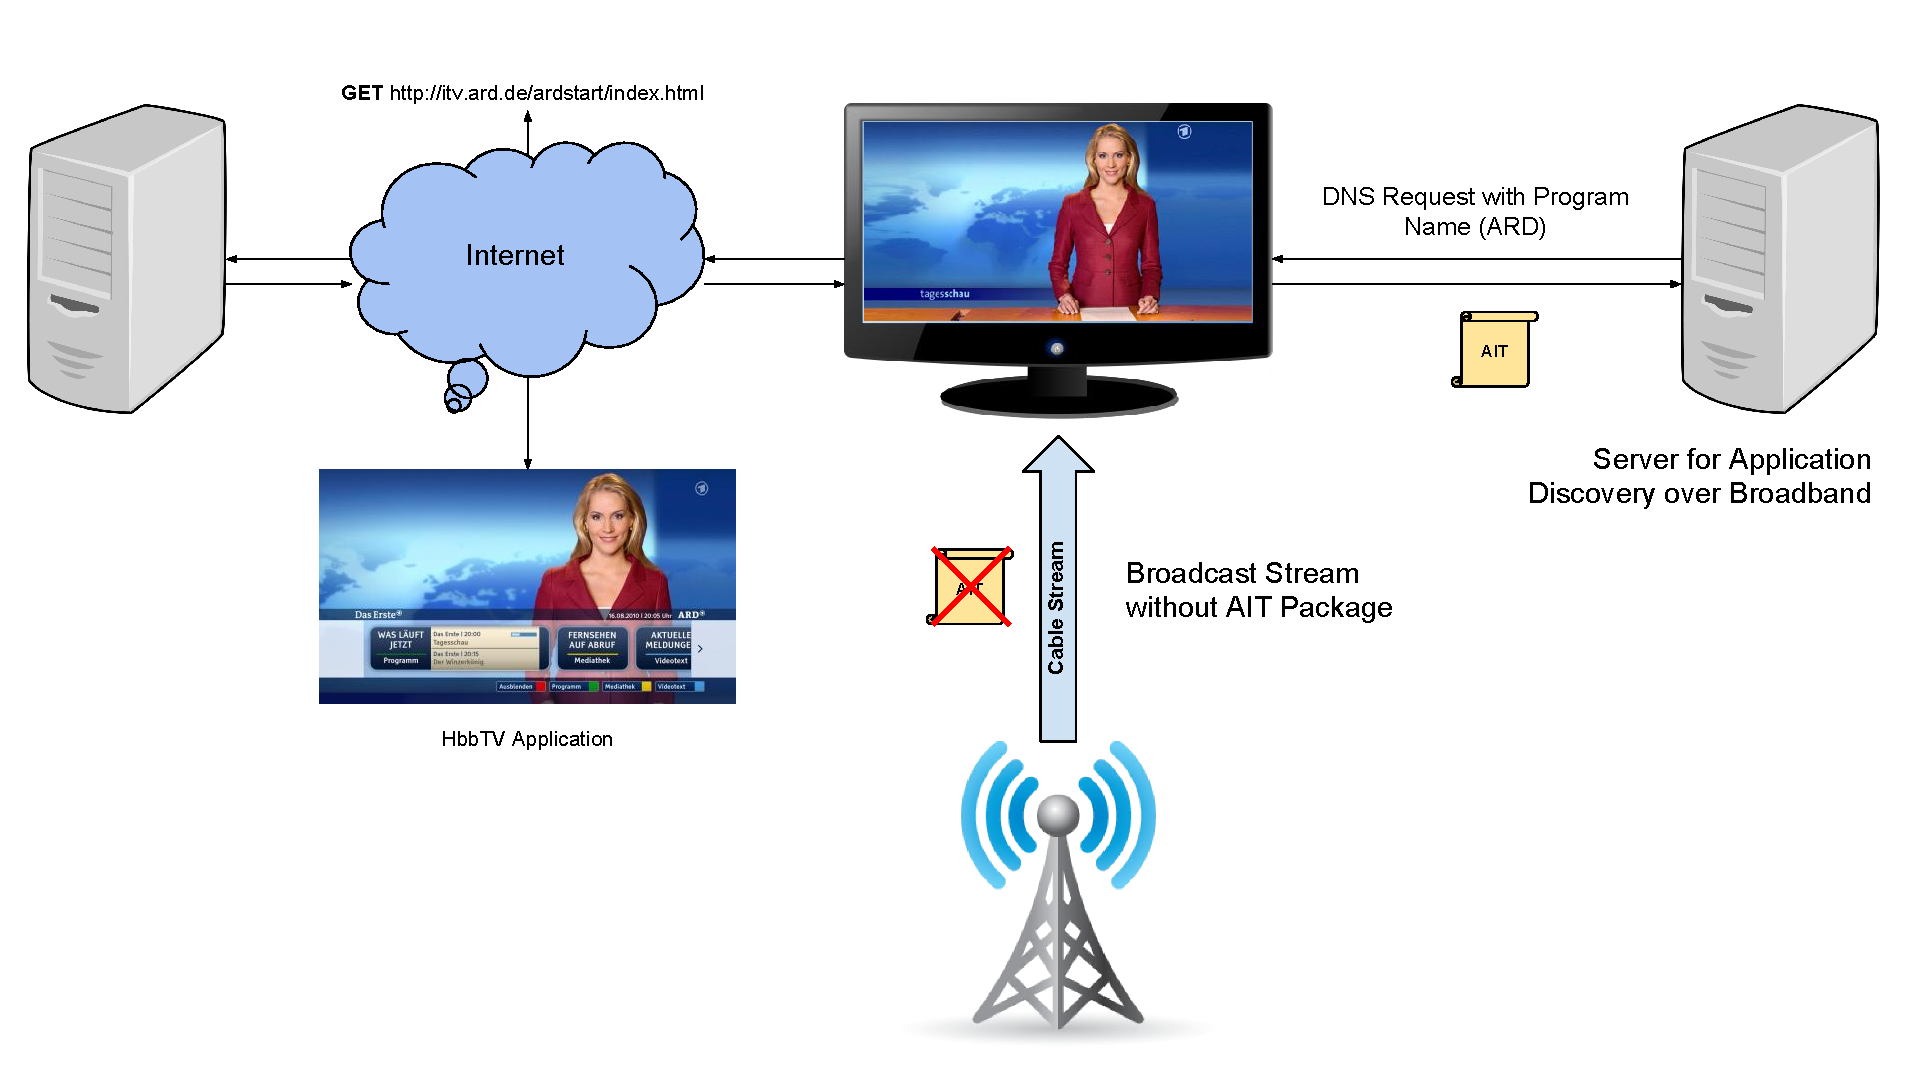
\includegraphics[width=15cm]{application_discovery_over_broadband.pdf}\\
  \caption{App delivery workflow of HbbTV applications}\label{fig:application_discovery_over_broadband}
\end{figure}

As described in Figure \ref{fig:application_discovery_over_broadband} the TV gets the AIT package
from a dedicated server based on the program name. Each broadcaster usually has their own DNS
root server and an own AIT server. However there is one main HbbTV DNS root server which routes the
DNS request from the TV to the server of the broadcaster.\\
Pay, cable, IPTV or Sat-Platform operators as mentioned above sometimes provide instead of HbbTV
their own service apps with own GUI. They usually require some sort of additional hardware which
don't support HbbTV. Even though the TV is connected to the internet and supports the standard
it is still not possible to open up an HbbTV application. As solution for this problem the
consortium around the standard invented the so called Operator Apps which allow to connect
operator and HbbTV applications on one Smart TV. The idea is that the user can switch between
both worlds as a functionality within the TV. An operator can become anyone who has a contract
with the TV manufacture. Each operator app has to authenticate to the TV to avoid abuse. Unlike
HbbTV applications and operator app can run in the background at all times and can display
messages on the display as well as overwrite key functions like \textit{''P+''} or \textit{''P-''}.
They open usually by pressing \textit{''EPG''} or \textit{''Menu''}. In the specification of
operator apps which is part of HbbTV verson 2 the consortium emphasized that operator and HbbTV
apps can live seamlessly together.\\
Looking back at the standard that was first specified 7 ago HbbTV has taken a very interesting
development. From being able to show more than a digital and interactive teletext to supporting
HTML5 and Second Screen it became quite comprehensive. This enables broadcasters to use this
service in a variety of ways.

\subsection{Example applications and Use Cases}

All these features allow broadcasters to implement not only an additional content outlet but also
to create tailored advertisment strategies to a specified audience. With methods like geotargeting
or targeted advertisment. Geotargeting can be used in HbbTV applications by leveraging a users
IP address in order show regional products or services. Combined with a broadcast stream it
enables interesting opportunities. In an advertisment campaign launched by Germans private
broadcaster RTL they promoted a pharmaceutical with help of an HbbTV app. The pharmaceutical
\textit{''Wick Medinait''} was advertised along with a banner that showed the regional weather
forecast. It had the effect that the HbbTV app banner supported the TV spot so that it increased
the impact of the advertisment itself.

\begin{figure}[htb]
  \centering
  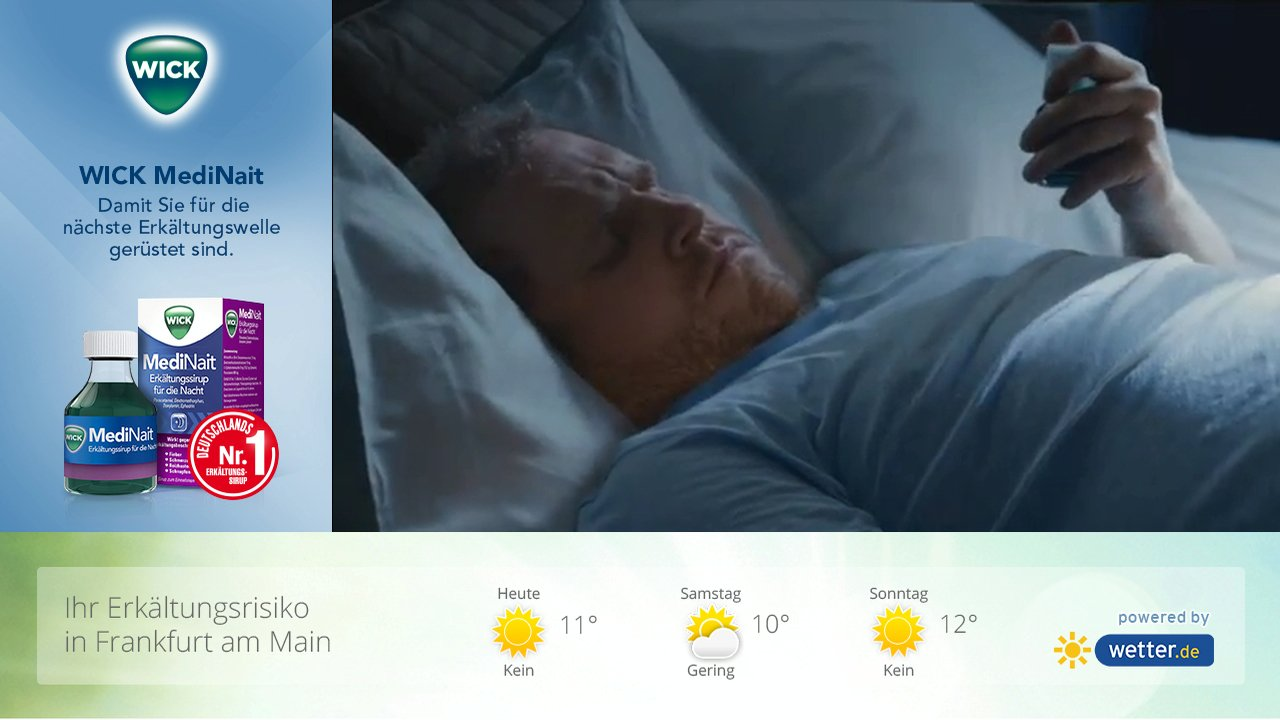
\includegraphics[width=10cm]{geotargeting.jpg}\\
  \caption{
    Use case of geotargeting via HbbTV\\
    {\tiny Image Source: https://goo.gl/rab8XD}
  }
  \label{fig:geotargeting}
\end{figure}

This is also called Addressable TV advertising. It \textit{''enable[s] advertisers to selectively
segment TV audiences and serve different ads or ad pods (groups of ads) within a common program or
navigation screen. Segmentation can occur at geographic, demographic, behavioral and (in some cases)
self-selected individual household levels [...]''}\cite{adrTV}.\\
Another interesting use case outside of advertisment is content authoring of HbbTV applications.
Usually an HbbTV application is a custom web app that is build to serve a specific content for
a service or show. Once you want to promote a new service or show it requires to build a new
app with new content. This takes time and cost money. A solution to this problem was adapted from
the web. By using a Content Management System (CMS) like Wordpress\footnote{\url{https://wordpress.org/}}
broadcaster can create or modify the content of their apps using a simple web interface.

\begin{figure}[htb]
  \centering
  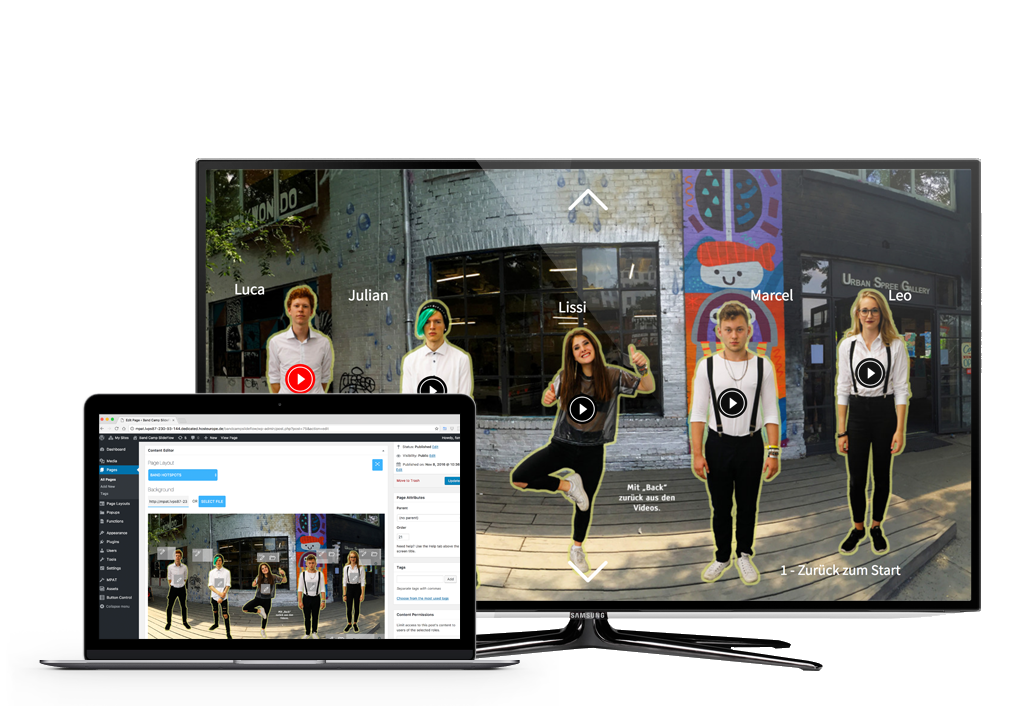
\includegraphics[width=10cm]{mpat.png}\\
  \caption{
    Modifying HbbTV content via a web interface
  }
  \label{fig:mpat}
\end{figure}

Figure \ref{fig:mpat} shows how this looks like with a tool called MPAT\footnote{\url{https://www.fokus.fraunhofer.de/en/fame/project/mpat}},
a project that was funded by the European Union and developed and led by Fraunhofer Fokus.
It uses Wordpress as CMS to enable authors to modify content, look or functionality of an HbbTV
app. Thanks to its plug\&play functionality the tool can easily add new features like Chat and Video or
Image Galleries without requiring someone to implement it. With that it reduces the risk of unexpected
behavior as this plugins are already tested against common Smart TV devices.

\subsection{HbbTV Runtime Environment\label{sec:hbbtvruntimeenvironment}}

- What's the lifetime cycle for HbbTV apps
- see spec (autoload etc.)

\subsection{Development of HbbTV Applications\label{sec:devofhbbtv}}

- How do engineer build HbbTV apps these days (show HbbTV app boilerplate)
- What are typical app structures
- What kind of tooling does already exist (HAT project)

\subsection{Available test solutions\label{sec:availabletestsolutions}}

- How do engineer ensure quality of HbbTV apps
- give a glimb of existing product and reference of chapter 6

\section{Test Automation\label{sec:testautomation}}

For internal references use the 'ref' tag of LaTeX. Technology B is similar to Technology A
as described in section \ref{sec:hbbtv}.

\subsection{How Test Automation Changed the Industry\label{sec:howitchanged}}

- Study cases of how current top companies test their apps (not necessarry HbbTV)
- demonstrate how similar apps get tested these days
- outline the gap between both worlds

\subsection{History of Automated Testing\label{sec:history}}

- How Selenium and Appium has evolved

\subsection{Webdriver Protocol\label{sec:webdriver}}

- What is it
- Where is it supported
- How does it differ from previous JSONWireProtocol

\subsection{Cloud Solutions\label{sec:cloud}}

- How to do test automation in big scale
- compare different types of cloud solutions

\subsection{Tooling\label{sec:tooling}}

- What tools to use to run test automation
- What are their scope and restrictions

\subsection{Analysis of Test Automation Demand for TVs\label{sec:testautomationontv}}

- How do devices differ
- only input remote control
- what could the future bring to us?

\section{Chrome Remote Debugging Protocol}

- What is it
- for what is it used for
- what about other browser (remotedebug.org)
- somethine from https://github.com/ChromeDevTools/awesome-chrome-devtools

\subsection{Functional Principles of modern Web Browser\label{sec:howbrowserwork}}

- How browser work

\subsection{Communication between Chrome DevTools Frontend and the Browser}

- How does the devtools frontend gets all the data from the browser
- why does it not affect the performance

\section{HbbTV and Web Platform Tests}

- How HbbTV devices get tested
- how other standards get tested
- validator (http://hbbtv-live.irt.de/validator/, http://ligada-validator.com/)
